%%%%%%%% ICML 2021 EXAMPLE LATEX SUBMISSION FILE %%%%%%%%%%%%%%%%%
\documentclass{article}
\usepackage[]{algorithm2e}
\usepackage{algorithmic}
\usepackage{algorithm}
% Recommended, but optional, packages for hs and better typesetting:
\usepackage{microtype}
\usepackage{graphicx}
\usepackage{amsmath}
\usepackage{appendix}
\usepackage{subfigure}
\usepackage{booktabs} % for professional tables
\usepackage{hyperref}
% Attempt to make hyperref and algorithmic work together better:
\newcommand{\theHalgorithm}{\arabic{algorithm}}
\usepackage{icml2021}
\usepackage{float}
\usepackage{enumitem}

\begin{document}
\twocolumn[
\icmltitle{Reinforcement Learning 2024
Assignment 3: Policy-based Reinforcement Learning}

\icmlsetsymbol{equal}{*}
\begin{icmlauthorlist}
\icmlauthor{Sherry Usman}{equal,to}
\icmlauthor{Qin Zhipei}{equal,to}
\icmlauthor{Megan Mirnalini Sundaram R}{equal, to}
\end{icmlauthorlist}

\icmlaffiliation{to}{Leiden University}

% You may provide any keywords that you
% find helpful for describing your paper; these are used to populate
% the "keywords" metadata in the PDF but will not be shown in the document
\icmlkeywords{Machine Learning, Deep Q-Learning, Experience Replay, Target Network}

\vskip 0.3in
]

\begin{abstract}

\end{abstract}

\section {Introduction}
In this paper we will delve into the Lunar Lander environment taken from the OpenAI Gym library. The Lunar Lander game is a classical reinforcement learning environment where the goal is to optimise the trajectory of a rocket such that it lands between the two flags.
In this paper we delve into the implementation of DQN in the CartPole environment. The CartPole is a classical reinforcement learning environment where the goal is to balance a pole on the cart, while  applying forces to the cart at the bottom (as shown in Figure 1) \citep{brockman2016openai}. While a number of different techniques can be used to solve this problem, our paper specifically concentrates on the use of DQNs. Through this paper, we hope to provide the specifications of various DQN models while also including the various exploration strategies that provide us the best exploration-to-exploitation ratio and also optimal hyper-parameters that will yield the best results. Furthermore, we hope to provide an extensive ablation study to help identify the impact of adding and removing certain components (specifically, experience replay and target network) on DQN's performance. \newline

\section{Framework}
\label{Introduction and General Strategy}

The CartPole environment poses unique challenges compared to the environments we have encountered previously. While the action space $A$ is still discrete with two potential actions (push left and push right), there is a continuous observation space/state space $S$ which includes the \textbf{cart position}, \textbf{cart velocity}, \textbf{pole angle} and \textbf{pole angular velocity}. A high-dimensional state space such as this makes the creation of a Q table/array storing the values for every state-action pair quickly infeasible. Thus, to tackle this problem we use DQNs which leverages the advantages of \emph{function approximation} to obtain q values. 

\begin{figure}[htbp]
\centering
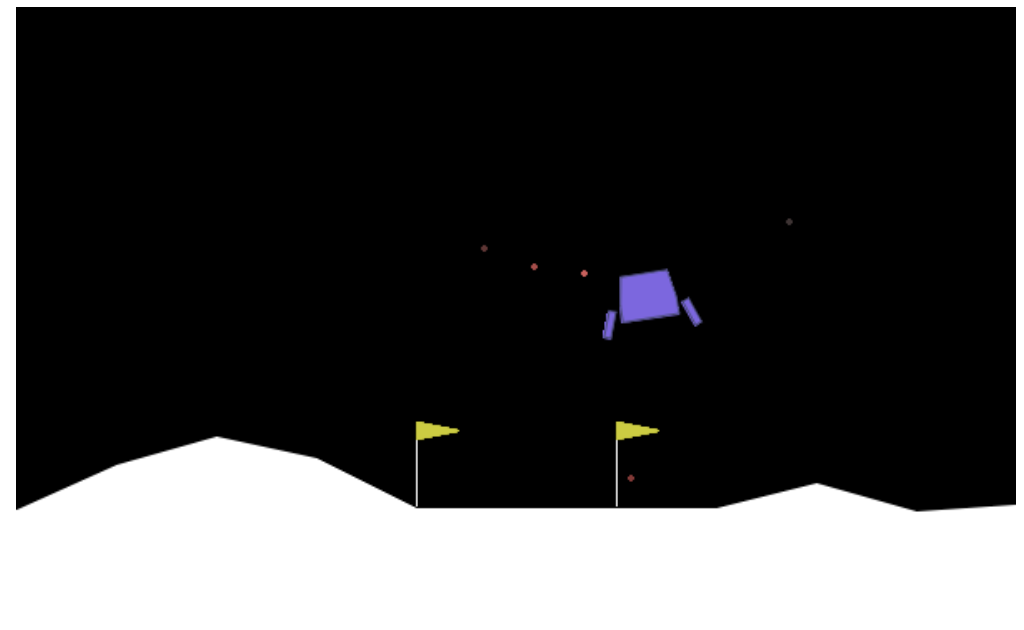
\includegraphics[width=0.6\linewidth]{Report/images/visualisation.png}
\caption{\label{fig:Visualization of the Cart-pole} A visualisation of the Lunar Lander problem}
\end{figure}



The action space of the lunar lander environment is shown below. 
As seen below there are 4 potential actions: 0,1,2 and 3. 

\begin{table}[htbp]
\centering
\begin{tabular}{|l|c|}
\hline
\textbf{Value} & \textbf{Action} \\
\hline
0  & Do nothing \\
\hline
1 & fire left orientation engine \\
\hline
2  & fire main engine \\
\hline
3 & fire right orientation engine  \\
\hline
\end{tabular}
\caption{Action Space}
\label{tab:hyper-parameters}
\end{table}

The observation space is an 8-dimensional vector, the positional coordinates of the lunar lander (x and y), its linear velocities in x and in y respectively, its angle, its angular velocities and two boolean values that represent whether each leg is in contact with the ground or not. 

\section{Policy-Based Reinforcement Learning}
The policies we looked at in the previous papers were \emph{value-based}. This means that they looked at state-value pairs in the environment and approximated the rewards of such pairs using different exploration strategies like Boltzmann or Epsilon-Greedy. Policy based reinforcement learning methods differ from value-based method as they do not utilize a value function to determine the next possible action. Used primarily in  continuous action space RL environments, policy based reinforcement learning methods use a parameterized policy function $\pi_\theta$ where $\theta$ represents the parameters of the function.
During training the agent iteratively interacts with the environment over multiple episodes. After a number of episodes the collected data known as the trajectory $\tau$ is evaluated to understand the performance of the policy. If $\tau$ yields high rewards then the parameters $\theta$ are adjusted in such a way that the likelihood of taking actions similar to the actions in this trajectory is increased. On the other hand if the trajectory $\tau$ yields lower rewards then the parameters $\theta$ are adjusted in such a way that the likelihood of taking actions similar to such actions is decreased. This process of iteratively evaluating the trajectories and updating the parameters according to the obtained rewards/losses helps to refine the policy to maximize cumulative rewards in the long run \cite{plaat-deeprl}.

There are a number of different policy-based reinforcement learning algorithms. However for this paper, we are limiting the scope of our research to the algorithms listed below: 

\begin{itemize}
\item REINFORCE
\item Actor-Critic
\item Actor-Critic with baseline subtraction
\item Actor-Critic with bootstrapping
\item Actor Critic with bootstrapping and baseline subtraction
\end{itemize}
These algorithms are discussed in detail below. 

\subsection{REINFORCE}
\quad REINFORCE is a commonly used Policy-based Reinforcement Learning algorithm which is also termed as a classic Monte-Carlo Policy Gradient algorithm. It learns from the collected episodes by estimating gradients throughout the agent trajectory. Because it needs a full trajectory in order to construct a sample space it is updated as an off-policy algorithm. \newline
\begin{equation}
\pi_\theta(a, s) = Pr(A_t = a | St = s, \theta_t = \theta)
\end{equation}
The equation above helps us recall the policy function $\pi_{\theta}(a, s)$ which indicates the probability of taking an action a in the state s with the parameters $\theta$. \newline
The REINFORCE algorithm optimises the policy function $\pi_{\theta}(a,s)$ by fine-tuning its parameters $\theta$ such that it increases the likelihood of actions in trajectories $\tau$ which lead to higher cumulative rewards. It does this by calculating the total expected rewards with respect to a particular parameter value $\theta$ and adjusting $\theta$ accordingly. Thus the parameters are updated as follows: \newline

1. We first calculate J($\theta$) which represents the expected cumulative rewards. 
\begin{equation}
J(\theta) = E[ \sum_{t=0}^{T-1}r_t + 1] 
\end{equation}

where $r_{t}$ indicates the reward obtained at time t for executing a certain action $a_t$ at state $s_t$.
Thus $\theta$ is optimised to be equal to the gradient ascent of the partial derivative with respect to $\theta$ of $J(\theta)$. Thus $\theta$ is updated as shown in the equation below. 
\begin{equation}
\theta = \theta + \frac{\mathrm{d}  }{\mathrm{d} \theta} J(\theta)
\end{equation}

The algorithm for REINFORCE can thus be defined as follows: 
\begin{algorithm}[htbp]
\caption{REINFORCE Algorithm}
\SetAlgoLined
\DontPrintSemicolon
\small % Set font size to small
\KwData{parameter $\theta$, policy function $\pi_\theta$, maximum timesteps $T$, number of episodes $E$}
\KwResult{Selected action}
Initialise $\theta$ arbitrarily\;\\
\For{$e = 1$ \KwTo $E$}{
    Initialise state $s$\;
    \For{$t = 1$ \KwTo $T-1$}{
     Sample action $a$ from $\pi_\theta$\;
    Execute action $a$ and get the next state $s_{t+1}$ and the observe reward $r_t$\; 
        \theta \leftarrow \theta + \alpha * \nabla_\theta log \pi_\theta(s_t, a_t) v_t 
    }
}
 Return parameter $\theta$\;
\end{algorithm}


%There are many variations of REINFORCE that can produce better results. 

%As mentioned above, the parameters of the policy is defined by $\theta$. Therefore, the quality of such parameters for the state to action probabilities for the policy is given by $J(\theta)$. To improve the gradient, the differential of the parameters are taken. 

%\newline The quality is given by $\mathbb{E}_\pi [ \sum _a q_\pi(S_t, a)\nabla_\pi(a|S_t, \theta)]$

%\newline The update of these functions happen in a Monte-Carlo function i.e., random sample. The function is updated after an entire trajectory/path is completed. Therefore, this happens in an off-policy way.  

\subsection{Actor-Critic Methods}
 Actor Critic methods are TD methods and have a separate memory structure to store the policy independent of the value function. Thus it has two  structures/neural networks: a policy structure known as an \emph{actor} and an estimated value function known as the \emph{critic}. While the actor follows the policy and takes actions according to the policy, the critic, typical of its name, criticises the actions taken by the actor in the form of a TD error. This scalar signal indicates whether the actions taken by the agent are better or worse than what the critic expected. The TD error can be evaluated as follows in the following equation: \newline
 $\delta_{t} = R_{t+1} + \gamma * V_t(S_{t+1})-V_t(S_t)$ \newline
 where $\delta_{t}$ is the temporal difference error at timestep $t$, $R_{t+1}$ is the reward for transitioning from state $S_t$ to the state $S_{t+1}$,  $\gamma$ is the discount factor, $V_{t}$ is the value function from the critic and $V_t(S_{t+1})$ is the estimated value of going to state $S_{t+1}$ while $V_t(S_t)$ is the estimated value of going to state $S_t$.  \newline 
 Thus, a positive TD error indicates that the transition from state $S_t$ to $S_{t+1}$ is fruitful/ has a positive reward while a negative TD error indicates that the transition from state  $S_t$ to $S_{t+1}$ to $S_{t+1}$ is not rewarding.
 \newline

 


\newline As used in REINFORCE, the policy gradient is given by 
\newline 
$\nabla_\theta J(\theta) = \mathbb{E}_\pi[\sum _{t=0}^{T-1} \nabla_\theta log\pi_\theta (a_t|s_t)G_t]$


\begin{figure}[htbp]
\centering
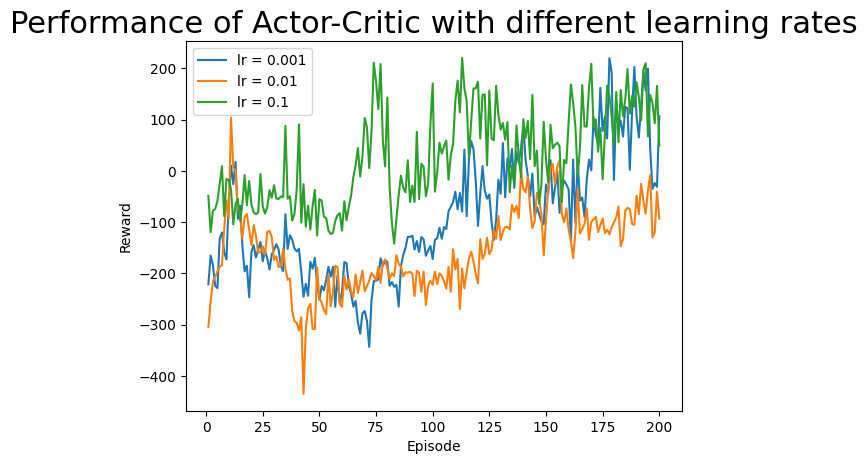
\includegraphics[width=1.2\linewidth]{Report/images/actor_critic_no_bs.png}
\caption{\label{fig:ActorCritic}The figure above shows the result of Actor Critic with different learning rates. As we can see, all learning rates show a rising trend of rewards, with the graph for learning rate 0.01 showing the most improvement}
\end{figure}



\subsubsection{Bootstrapping}
Actor Critic with bootstrapping is a particular actor-critic algorithm that combines the benefits of both value based (using state-action pairs) and policy based methods. Thus the inclusion of elements from value-based reinforcement learning bootstraps or supports the policy-based traditional Actor-critic method by counteracting the low bias and high variance. It combines the advantage of having a low variance from the value method, and the advantage of having a high bias from the policy method.
Similar to the traditional actor critic method, there is an actor who learns the policy and there is a critic which criticises/evaluates the rewards gained from following the policy (the value of particular state-action pairs Q(s,a)) . However, in the case of Actor Critic with bootstrapping, the critic uses bootstrapping to update the value Q of the state-action pairs, harking back to value-based methods. \newline 
particular state-action pairs  the actions taken by teh agent oin the form of a TD error. However, the critic 
However, there might be high variance in the rewards and gradient estimate. To counteract this, bootstrapping is used. 

\subsubsection{Baseline Subtraction}
Actor-Critic algorithms could also employ baseline subtraction which is a technique used to reduce the variance by using a baseline. We recall the previous policy gradient function denoted by $\nabla_\theta J(\theta) = \mathbb{E}_\pi[\sum _{t=0}^{T-1} \nabla_\theta log\pi_\theta (a_t|s_t)G_t]$. By subtracting a baseline $b(s_t)$ from the cumulative reward helps reduce make them smaller and more stable, reducing variance. The updated policy gradient function after baseline subtraction is shown below. 

$\nabla_\theta J(\theta) = \mathbb{E}_\pi[\sum _{t=0}^{T-1} \nabla_\theta log\pi_\theta (a_t|s_t)G_t - b(s_t)]$



\subsubsection{Bootstrapping and Baseline Subtraction}


\section{Goals Achieved}
\subsection{Effects of policy gradients on variance}
\subsection{Effects of bootstrapping on the policy gradients}
\subsection{Comparison of Performance}
\subsection{Effect of entropy regularization on performance}

\bibliography{Report/references}
\bibliographystyle{Report/reference_style}
\end{document}

